\documentclass[11pt]{article}
\usepackage[margin=1in]{geometry}
\usepackage{../../styles/isaiah}
\usepackage{fontspec}
\usepackage{bidi}
\usepackage{../../styles/components/leftRightGrid}
\begin{document}

% Isaiah Context Grid
\leftRightGrid{2}{Isaiah 6-9:7}{
    \textbf{\large Isaiah 6}

    \textit{Isaiah's Call \& \\Commission}
}{
    \textbf{\large Isaiah 7}

    \textit{Immanuel}
}{
    \textbf{\large Isaiah 8}

    \textit{Maher-shalal-hash-baz}
}
{
    \textbf{\large Isaiah 9:1-7}

    \textit{The Prince of Peace}
}

% Overview of Isaiah 7
\begin{overview}{Isaiah 7:1-25 — Overview}

\overviewsection[0]{%
\textbf{Verses 1-6: Problem of Potential Future Judgment}
\begin{itemize}
    \item \highlightorange{Syria} and \highlightbrown{Israel} alliance threatens Judah
    \item Ahaz and people tremble with fear
\end{itemize}
}

\overviewsection[1]{%
\textbf{Verses 7-9: God will protect – have strong faith}
\begin{itemize}
    \item Yahweh through Isaiah speaks
    \item Faith requirement: "If you are not firm in faith, you will not be firm at all"
\end{itemize}}

\overviewsection[1]{%
\textbf{Verses 10-17: Faith test – Immanuel / God is with us}
\begin{itemize}
    \item Yahweh through Isaiah speaks
    \item God gives the Immanuel sign
\end{itemize}
}

\overviewsection[0]{%
\textbf{Verses 18-25: Problem of Sure Future Judgment}
\begin{itemize}
    \item \highlightred{In that day} - repeated phrase marking divine intervention
    \item Assyrian invasion will devastate Judah
\end{itemize}
}

\end{overview}

\newpage

% Section 1: Verses 1-6 - Chiastic Structure
\begin{chiasticoutline}[Isaiah 7:1-6]{.95em}{2em}


    \chiasticverse[A]{0}{
        \versenum{1} In the days of Ahaz the son of Jotham, son of Uzziah, king of Judah, \highlightorange{Rezin the king of Syria} and \highlightbrown{Pekah \sectionwordfootnote{the son of Remaliah}{Pekah not mentioned by name here on -- likely because he was a usurper, not of royal blood} the king of Israel} came up to Jerusalem to wage war against it, but could not yet mount an attack against it.
    }
    
    \chiasticverse[B]{1}{
        \versenum{2a} When the house of David was told, "\highlightorange{Syria} is in league with \highlightbrown{Ephraim}," 
    }

    \chiasticverse[C]{2}{
        \versenum{2b} the heart of Ahaz and the heart of his people shook as the trees of the forest shake before the wind.
    }

    \chiasticverse[D]{3}{
        \versenum{3} And the LORD said to Isaiah, "Go out to meet Ahaz, you and Shear-jashub your son, at the end of the conduit of the upper pool on the highway to the Washer's Field.
    }
    
    \chiasticverse[C']{2}{
        \versenum{4} And say to him, 'Be careful, be quiet, do not fear, and do not let your heart be faint because of these two smoldering stumps of firebrands, because of the fierce anger of \highlightorange{Rezin} and \highlightorange{Syria} and \highlightbrown{the son of Remaliah}.
    }
    
    \chiasticverse[B']{1}{
        \versenum{5} Because \highlightorange{Syria}, with \highlightbrown{Ephraim} and \highlightbrown{the son of Remaliah}, has devised evil against you, saying,
    }
    
    \chiasticverse[A']{0}{
        \versenum{6} "Let us go up against Judah and terrify it, and let us conquer it for ourselves, and set up the son of \sectionwordfootnote{Tabeel}{Good for Nothing} as king in the midst of it,"
    }

\end{chiasticoutline}

\newpage

% Section 2: Verses 7-9 - Chiastic Structure
\begin{chiasticoutline}[Isaiah 7:7-9]{.95em}{2em}

    \chiasticverse[A]{0}{
        \versenum{7} thus says the Lord GOD: "It shall not stand, and it shall not come to pass.
    }
    
    \chiasticverse[B]{1}{
        \versenum{8a} For the head of \highlightorange{Syria} is Damascus, and the head of Damascus is \highlightorange{Rezin}. 
    }
    
    \chiasticverse[C]{2}{
        \versenum{8b} And within sixty-five years \highlightbrown{Ephraim} will be shattered from being a people.
    }
    
    \chiasticverse[B']{1}{
        \versenum{9a} And the head of \highlightbrown{Ephraim} is Samaria, and the head of Samaria is \highlightbrown{the son of Remaliah}.
    }
    
    \chiasticverse[A']{0}{
        \versenum{9b} If you are not firm in faith, you will not be firm at all.'"
    }

\end{chiasticoutline}



% Section 3: Verses 10-17
\begin{biblicaloutline}[Isaiah 7:10-17]

    \subsectionheader{The Sign Offered (10-12)}
    
    \begin{versesection}{2em}
        \versenum{10} Again the LORD spoke to Ahaz: \versenum{11} "Ask a sign of the LORD \highlightyellow{your God}; let it be deep as \sectionwordfootnote{Sheol}{The grave/pit. Deep in the earth where the dead are buried.} or high as heaven." \versenum{12} But Ahaz said, "I will not ask, and I will not put the LORD to the test."
    \end{versesection}
    
    \subsectionheader{The Sign Given (13-17)}
    
    \begin{versesection}{2em}
        \versenum{13} And he said, "Hear then, O house of David! Is it too little for you to weary men, that you weary \highlightyellow{my God} also? \versenum{14} Therefore the Lord himself will give you a sign. Behold, the virgin shall conceive and bear a son, and shall call his name \highlightaqua{Immanuel}. \versenum{15} He shall eat curds and honey when he knows how to refuse the evil and choose the good. \versenum{16} \highlightgreen{For before the boy knows how to} refuse the evil and choose the good, the land whose two kings you dread will be deserted. \versenum{17} The LORD will bring upon you and upon your people and upon your father's house such days as have not come since the day that \highlightbrown{Ephraim} departed from Judah—the king of Assyria."
    \end{versesection}

\end{biblicaloutline}

\vspace{3em}
{\large\bfseries Will not Put to the Test?}
\vspace{1em}

It seems like Ahaz is doing something nobel here by refusing to test the Lord (as commanded in Deut 6:16).

But, in the Hebrew ordering of the Bible, the TaNaK, Isaiah comes right after 2 Kings. In 2 Kings 16:7-9, we see that Ahaz actually \textit{did} put the Lord to the test by asking Tiglath-Pileser III of Assyria to come and help him against the alliance of Syria.
\\\\
John Oswalt has referred to this as 3 mice getting into a fight and one of them going to ask the cat for help! Ahaz, the wicked king, is showing his lack of trust in a passage here in Isaiah when trust in Yahweh is central.

\newpage

{\large\bfseries Virgin vs Young Woman}
\vspace{1em}

\hebrewword{Virgin}{עַלְמָה}{al.mah}{young woman of marriable age}

In the Hebrew text, the word used for "virgin" in verse 14 is \textit{almah}, which simply means "young woman of marriable age." However, when the Hebrew Bible was translated into Greek (called the Septuagint), the translators chose to use the word \textit{parthenos}, which specifically refers to someone who has never had sexual relations or borne children. This translation choice was significant for how later readers understood this prophecy.
\\\\\\\\
Matthew references this very passage when describing the birth of Jesus:
\\
\begin{quote}
\textit{"All this took place to fulfill what the Lord had spoken by the prophet: 'Behold, the virgin shall conceive and bear a son, and they shall call his name \highlightaqua{Immanuel}' (which means, \highlightaqua{God with us})."} \\
\hfill --- Matthew 1:22-23
\end{quote}
{\vspace{1em}}
So why would Matthew quote this text with the word "virgin"? Or better yet, why would the Greek translators of the Hebrew Bible use "parthenos" instead of the other word for "young woman"? What is this all referring to and how does this text actually predict the coming Messiah at all?


\vspace{3em}
{\large\bfseries The Virgin Birth Prophecy}
\vspace{1em}

There is a lot of comparisons in this and surrounding passages about Ahaz in Isaiah when compared to his son, Hezekiah in chapters 36-39.

Much of this insight comes from Bible Scholar Tim Mackie who also credits Jacob Stromberg. Here's a chart from them, in fact, comparing these two stories from the kings:

\begin{center}
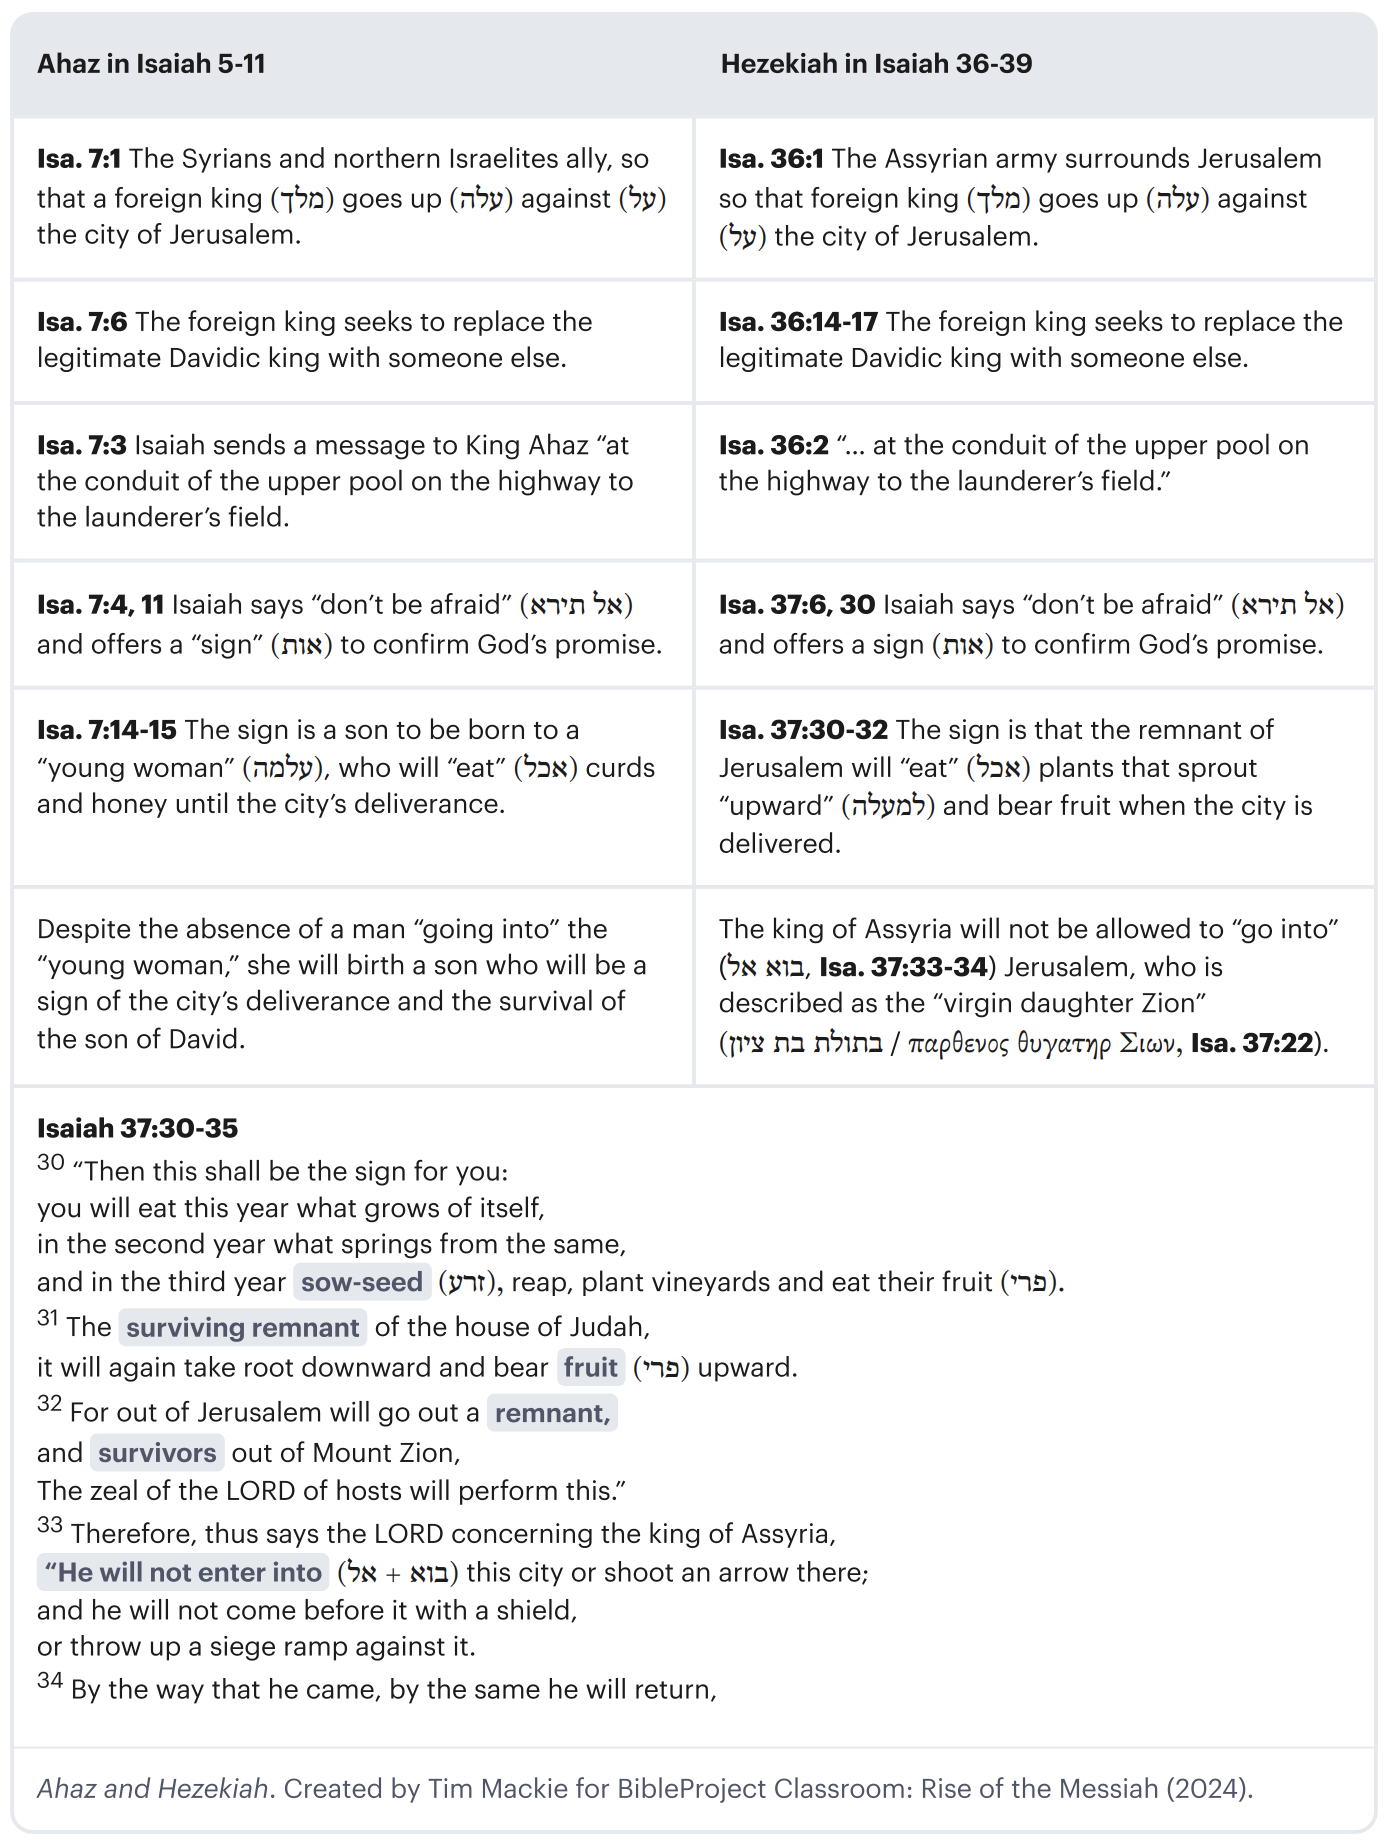
\includegraphics[width=1\textwidth]{ahaz-hezekiah-comparison.png}
\end{center}
{\vspace{1em}}
In both of these stories, we have a King who's worried about a raging army about to go against it and "break it open" in order to install a puppet king.
\\\\
God offers them both a sign of His promise of protection, even though Ahaz refuses.
\\\\
This Immanuel sign is put on analogy to the surviving remnant in Isaiah 37:30-35. Even though the "Virgin daughter Zion" is not able to be entered, there will still be a fruitful "surviving remnant" coming forth from it as a sign of salvation.
\\\\
This is exactly what the last few chapters of this whole book is about – a glorious surviving remnant worshipping Yahweh in a future glorious Zion! All of this, as we'll read later in Isaiah, is made possible by the coming Suffering Servant. The King of David. The Messiah.


% Section 4: Verses 18-25
\begin{biblicaloutline}[Isaiah 7:18-25]

    \begin{versesection}{2em}
        \versenum{18} \highlightred{In that day} the LORD will whistle for the fly that is at the end of the streams of Egypt, and for the bee that is in the land of Assyria. \versenum{19} And they will all come and settle in the steep ravines, and in the clefts of the rocks, and on all the \highlightgreen{thornbushes}, and on all the pastures.
        
        \versenum{20} \highlightred{In that day} the Lord will shave with a razor that is hired beyond the River—with the king of Assyria—the head and the hair of the feet, and it will sweep away the beard also.

        \versenum{21} \highlightred{In that day} a man will keep alive a young cow and two \highlightgray{sheep}, \versenum{22} and because of the abundance of milk that they give, he will eat curds, for everyone who is left in the land will eat curds and honey.
        
        \versenum{23} \highlightred{In that day} every place where there used to be a thousand vines, worth a thousand shekels of silver, will become \highlightgreen{briers and thorns}. \versenum{24} With bow and arrows a man will come there, for all the land will be \highlightgreen{briers and thorns}. \versenum{25} And as for all the hills that used to be hoed with a hoe, you will not come there for fear of \highlightgreen{briers and thorns}, but they will become a place where cattle are let loose and where \highlightgray{sheep} tread.
    \end{versesection}

\end{biblicaloutline}

\vspace{3em}
{\large\bfseries Untamable Land}
\vspace{1em}

Having land that used to be able to be worked ("hoed with a hoe"), but now they are full with briers and thorns is reminiscent of the fall as mentioned in Genesis 3:17-19:
\\\\
\begin{quote}
\textit{"And to Adam he said, 'Because you have listened to the voice of your wife and have eaten of the tree of which I commanded you, "You shall not eat of it," cursed is the ground because of you; in pain you shall eat of it all the days of your life; \highlightgreen{thorns and thistles} it shall bring forth for you; and you shall eat the plants of the field. By the sweat of your face you shall eat bread, till you return to the ground, for out of it you were taken; for you are dust, and to dust you shall return.'"} \\
\hfill --- Genesis 3:17-19
\end{quote}
\vspace{1em}

This also fits in with the rest of the imagery in v23-25 too between the initially abundant places that now are filled with violence and where the animals are not subdued (Gen 1:28).

Jerusalem's flourishing can be spoken of like Eden and it's destruction can be spoken of like the end of the world throughout the prophets. What God is doing through these people has worldwide implications for humanity's quest to return to Eden.

\end{document}